\section{PreGLAM and Multi-Track Music Machine}

\subsection{PreGLAM}

The Predictive Gameplay-based Layered Affect model (or short: PreGLAM)
was developed to be integrated flexibly into the design process of a 
game \cite{plut2023preglam}. PreGLAM is an artificial cognitive agent
designed to replicate the real-time emotional perceptions of a biased 
game spectator \cite{plut2023preglam}. PreGLAM calculates an estimation
of the game spectator's perceived emotion, which is based on the 
events in the game and other variables \cite{plut2023preglam}.

The PreGLAM models a spectator who has a certain game outcome as
a desire, but PreGLAM itself is not capable of affecting the gameworld
\cite{plut2023preglam}. The authors of PreGLAM modeled with the desire
of the player winning the game. They also state that there could 
be any quantifiable outcome used \cite{plut2023preglam}.

\subsubsection{Architecture}

\begin{figure}[h]
    \centering
    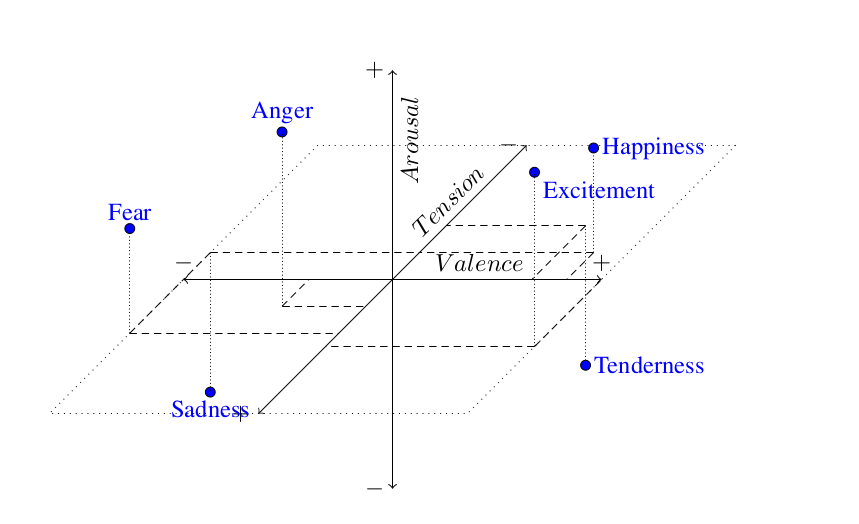
\includegraphics[width=\linewidth]{images/vat_model.png}
    \caption{3-Dimensional VAT Model of Affect, with example emotion categories placed for reference \cite{plut2023preglam}}
    \label{fig:vat_model}
\end{figure}

PreGLAM uses VAT model of affect \cite{plut2023preglam}. It has the dimensions
Valence, Arousal and Tension, as you can see in \Cref{fig:vat_model}. 

The authors describe Valence as a description of the current mood, whether it
is positive or negative \cite{plut2023preglam}. For instance, if a racing
game is played, and the own car passes another car which increases
the own car's position, or the own car crashes another car, the affect might be 
positive \cite{plut2023preglam}.
Nevertheless, getting hit by a car or being passed by someone else could 
possibly decrease the Valence value \cite{plut2023preglam}.

The Arousal in this context sometimes is paraphrased as "activity" or "energy", 
simulates the activation, or the intensity of an emotion \cite{plut2023preglam}.
High arousal emotions are emotions like excitement and fear, low arousal emotions
are emotions like calmness and sadness \cite{plut2023preglam}. 

\begin{figure}[h]
    \centering
    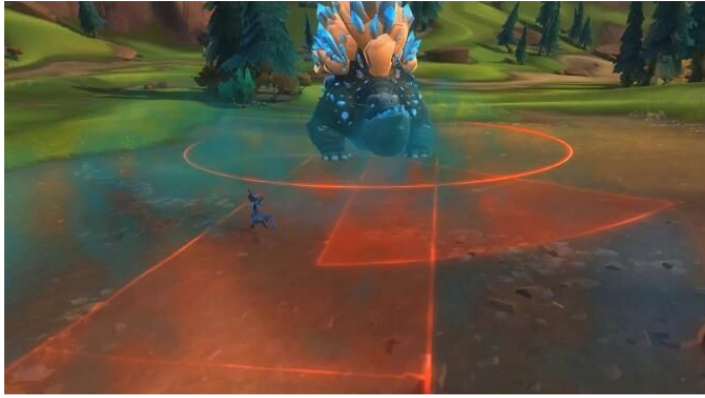
\includegraphics[width=\linewidth,height=4cm]{images/wildstar_attack_indicator.png}
    \caption{Attack telegraphs from Wildstar \cite{nixius2014wildstartelegraph}. The red areas indicate that an attack is coming soon (Figure and caption from \cite{plut2023preglam})}
    \label{fig:wildstar_indicator}
\end{figure}

The Tension involves the prospect or prediction of a future event
\cite{plut2023preglam}. It may be high if the next event might
be positive, but also negative in the case of a negative event
\cite{plut2023preglam}. An example of a future event can be seen
in \Cref{fig:wildstar_indicator}. It shows a set of attack telegraphs
from the MMO wildstar \cite{nixius2014wildstartelegraph} which 
communicate an event of incoming attack to the 
player\cite{plut2023preglam}. This may increase the tension, which
can lead the player to prevent or dodge the incoming attack 
\cite{plut2023preglam}.

Next to the gameplay desire the player can have, PreGLAM
also takes a set of events as input, which are annotated based
on how they affect the given desire, how strong their effect
on the desire is, and the values of variables which provide the 
gameplay context \cite{plut2023preglam}.

PreGLAM overlays its event-focused emotion rating model with an ambient mood score to generate a single affect score per dimension every 250 ms \cite{plut2023preglam}. PreGLAM calculates an emotion score from both events that have already occurred and predicted events \cite{plut2023preglam}. In addition, PreGLAM scales the emotion scores over time to reflect the ebb and flow of emotions over time \cite{plut2023preglam}.



\subsection{Multi-Track Music Machine}

\begin{figure}[h]
    \centering
    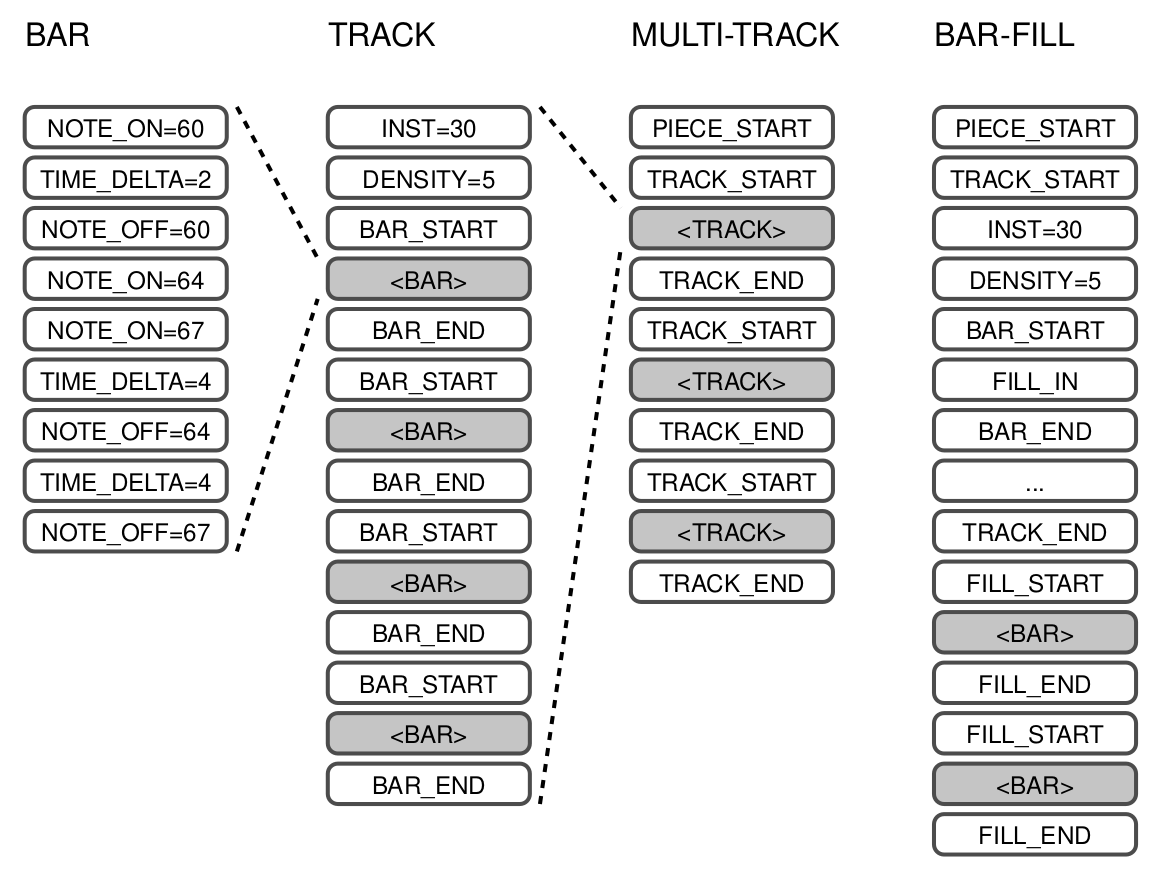
\includegraphics[width=\linewidth]{images/bar_fill_multi_track.png}
    \caption{The MultiTrack and BarFill representations are shown. The BAR tokens cor-
respond to complete bars, and the TRACK tokens correspond to complete tracks. (Figure and caption from \cite{ens2020mmm})}
    \label{fig:multi_track_figure}
\end{figure}

The Multi-Track Music Machine (MMM) was developed by Jeff Ens and Philippe Pasquier and is a generative music system that uses the Transformer architecture \cite{vaswani2017transformer} and is able to generate multi-track-music \cite{ens2020mmm}.

\subsubsection{Architecture and MultiTrack representation}

The representation of Tracks, Multi-Tracks, Bars and the Bar-Fill can be seen in \Cref{fig:multi_track_figure}.
The Bar representation consists of 128 NOTE\_ON tokens, 128 NOTE\_OFF tokens and 
48 TIME\_SHIFT tokens \cite{ens2020mmm}. The authors state
that due to the fact that musical events are quantised using 12 subdivisions per beat, the 48 used TIME\_SHIFT tokens
can be used for any rhytmic unit from
sixteenth note triplets to a full 4-beat
bar of silence \cite{ens2020mmm}. A bar 
starts with a BAR\_START token and ends
with a BAR\_END token \cite{ens2020mmm}. 

Tracks in this representation contain a sequence of bars and start with a 
TRACK\_START token and end with a TRACK\_END token \cite{ens2020mmm}.
After the TRACK\_START token, the track itself begins with the INSTRUMENT token \cite{ens2020mmm}.
It is used to specify the MIDI program that is used to play the notes on a 
certain track \cite{ens2020mmm}. There are 128 different INSTRUMENT tokens \cite{ens2020mmm}.
After the INSTRUMENT token follows the DENSITY\_LEVEL token, which specifies the note 
density of the track that is currently played \cite{ens2020mmm}.

A piece consists of multiple tracks and begins with a PIECE\_START token,
where bars are put into tracks, and tracks are put into a piece \cite{ens2020mmm}.
A PIECE\_END token is not used within a piece, because a piece contains exactly 
n tracks \cite{ens2020mmm}.

With the help of the MultiTrack representation, the model learns to make the generation
of every track dependent of of the pre-generated track \cite{ens2020mmm}.
During the generation, the process allows for a subset of the musical material to be
fixed while generating additional tracks \cite{ens2020mmm}.

Nevertheless, the MultiTrack representation introduced by Ens and Pasquier only offer control at the track level, but not at the bar level, except the model is asked to complete the remaining bars of a track \cite{ens2020mmm}. In order to achieve this, 
the authors remove all the bars to be predicted and replace each of them with a
FILL\_PLACEHOLDER token \cite{ens2020mmm}. 

After the removal, the removed bars are inserted at the end of a track, more specifically,
after the last TRACK\_END token \cite{ens2020mmm}. As the bars get inserted in the same 
order they got removed, they get wrapped with FILL\_START and FILL\_END tokens instead of 
BAR\_START and BAR\_END token \cite{ens2020mmm}. The authors call the resulting 
representation the BarFill representation \cite{ens2020mmm}.

\subsubsection{Training of MMM}

The authors use the Lakh MIDI Dataset \cite{raffel2016learning} for training their system \cite{ens2020mmm}. According to the authors, the training is done on a GPT2 model from 
Radford et al. \cite{radford2019language}, together with the HuggingFace Transformers
library of Wolf et al. \cite{wolf2019huggingface} using 8 attention heads, 6 layers, an
embedding size of 512 and an attention window of 2048 \cite{ens2020mmm}.

\subsection{PreGLAM-MMM}

For evaluation purposes, the authors of \cite{plut2022preglam} used the PreGLAM
emotion model \cite{plut2023preglam} and the Multi-Track Music 
Machine \cite{ens2020mmm} in their own game called Galactic Defense \cite{plut2022preglam}.


Galactic Defense is an action-RPG game, in which the player utilizes a set of
abilities, which are used to defeat a set of enemy units 
utilizing a recharging but limited resource pool, where he has 
to take care to not use certain abilities while beeing attacked \cite{plut2022preglam}.

\begin{figure}[h]
    \centering
    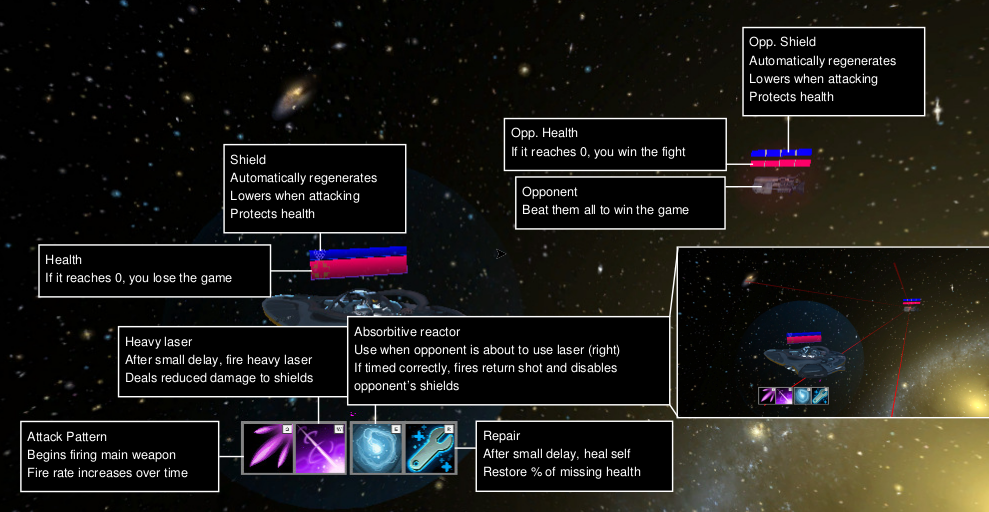
\includegraphics[width=\linewidth]{images/tutorial_gal_def.png}
    \caption{Tutorial scene of Galactic Defense \cite{plut2022preglam}}
    \label{fig:tutorial_gal_def}
\end{figure}

While playing, the player controls a spaceship, and the opponents
are AI-controlled spaceships, which the player has to defeat \cite{plut2022preglam}. The player's abilities contain four kinds of 
moves, shown in Fig. \Cref{fig:tutorial_gal_def} \cite{plut2022preglam}.
Also belonging to the resources, the player contains a shield, which is 
deactivated during the usage of an ability \cite{plut2022preglam}. Two of the 
player’s abilities are interruptible: the heavy laser and the repair ability. 
And if the player uses one of those abilities, either the heavy laser
or the repair ability, the player is more vulnerable and receives more 
damage from the enemy ships \cite{plut2022preglam}.
The player has to make tactical decisions within the game with
using his four types of moves \cite{plut2022preglam}.

There is a set of events that can happen within the game, which 
can have effect on the player's affect of emotions for the PreGLAM
model, as shown in \Cref{fig:emotion_table}. The table shows the base values for the emotional 
perceptions associated with each event, bzw. Emotionally Evocative Game Events, for short EEEG \cite{plut2023preglam}\cite{plut2022preglam}. These values are based on an initial unit of 1 and represent the 
intensity of the emotional response to the EEGE \cite{plut2022preglam}. All intensity modifiers are presented as percentages 
that scale the emotional values between 100 and 200\% \cite{plut2022preglam}. Tension is only calculated for prospective events, as tension arises from the prospect of events \cite{plut2022preglam}. An example of this is the "Player Shield Down"
EEGE, which has base values of -2 Valence, 1 Arousal, and 2 Tension \cite{plut2022preglam}. These values are modified based on 
how much health the player has left \cite{plut2022preglam}. For example, if the player is at 50\% of their maximum health and 
is expected to lose their shield, the output values scale to 150\% of their base value, and the output
values at the time the shield is expected to fall are 3 Valence, 1.5 Arousal, and 3 Tension \cite{plut2022preglam}. During 
actual gameplay, these values are additionally scaled over time \cite{plut2022preglam}.




\begin{figure}[h]
    \centering
    \scriptsize % Even smaller font size
    \begin{tabular}{|>{\centering\arraybackslash}m{2cm}|>{\centering\arraybackslash}m{0.7cm}|>{\centering\arraybackslash}m{0.7cm}|>{\centering\arraybackslash}m{0.7cm}|>{\centering\arraybackslash}m{2cm}|}
    \hline
    \textbf{Event} & \textbf{Valence} & \textbf{Arousal} & \textbf{Tension} & \textbf{Modifiers} \\ \hline
    P. complete atk combo & 1 & 1 & 1 & Missing O. shield \\ \hline
    P. heavy atk & 1 & 1 & 1 & Missing O. health \\ \hline
    O. atk combo & 1 & 1 & 1 & Missing P. shield \\ \hline
    O. heavy atk & -2 & 1 & 2 & Missing P. health, Parry active \\ \hline
    P. shields down & -2 & 1 & 2 & Missing P. health \\ \hline
    O. shields down & 2 & 1 & 2 & Missing O. health \\ \hline
    P. exploit O. disable & 3 & 1 & 2 & Missing O. health \\ \hline
    P. death & -3 & 1 & 3 & P. shield recharge time \\ \hline
    O. death & 3 & 1 & 3 & O. shield recharge time \\ \hline
    P. heal & 2 & 1 & 2 & Missing P. health \\ \hline
    O. heal & -2 & 1 & 2 & Missing O. health \\ \hline
    \end{tabular}
    \caption{Emotionally evocative events in GalDef \cite{plut2022preglam}. Player is shortened with P. and opponent is shortened with O. \cite{plut2022preglam}}
    \label{fig:emotion_table}
\end{figure}

To conclude, Their system used in 
Galactic Defense consists of an emotion model called PreGLAM from \cite{plut2023preglam},
the MultiTrack Music Machine from \cite{ens2020mmm}.

